%
% 計測自動制御学会システム・インテグレーション部門学術講演会2012原稿サンプルファイル
%                                           October 4, 2012
% Based on 計測自動制御学会システム・情報部門学術講演会2012原稿サンプルファイル
%                                           April 28, 2012
% Based on 第7回計測自動制御学会制御部門大会原稿サンプルファイル
%                                           October 18, 2007
% Based on 第5回計測自動制御学会制御部門大会原稿サンプルファイル
%            近野敦 konno@space.mech.tohoku.ac.jp    March 05, 2005
%

\documentclass[10pt,a4paper]{jarticle}
\usepackage{docmute}
\usepackage{tc2016_utf}
\usepackage[dvipdfmx]{graphicx,color}
\usepackage[fleqn]{amsmath}
\usepackage{algorithm,algorithmic}
\usepackage{amssymb,epsfig}
\usepackage{ascmac}

\usepackage{url}
\usepackage{bm}
\usepackage{ascmac}
\usepackage{pifont}
%\usepackage{multirow}
\usepackage{enumerate}
%\usepackage{cases}
\usepackage{type1cm}
\usepackage{here}
\usepackage{secdot}
\sectiondot{subsection}
\sectiondot{subsubsection}

\DeclareRelationFont{JY1}{mc}{it}{}{OT1}{cmr}{it}{}
\DeclareRelationFont{JT1}{mc}{it}{}{OT1}{cmr}{it}{}
\DeclareFontShape{JY1}{mc}{m}{it}{<5> <6> <7> <8> <9> <10> sgen*min
    <10.95><12><14.4><17.28><20.74><24.88> min10
    <-> min10}{}
\DeclareFontShape{JT1}{mc}{m}{it}{<5> <6> <7> <8> <9> <10> sgen*tmin
    <10.95><12><14.4><17.28><20.74><24.88> tmin10
    <-> tmin10}{}
\DeclareRelationFont{JY1}{mc}{sl}{}{OT1}{cmr}{sl}{}
\DeclareRelationFont{JT1}{mc}{sl}{}{OT1}{cmr}{sl}{}
\DeclareFontShape{JY1}{mc}{m}{sl}{<5> <6> <7> <8> <9> <10> sgen*min
    <10.95><12><14.4><17.28><20.74><24.88> min10
    <-> min10}{}
\DeclareFontShape{JT1}{mc}{m}{sl}{<5> <6> <7> <8> <9> <10> sgen*tmin
    <10.95><12><14.4><17.28><20.74><24.88> tmin10
    <-> tmin10}{}
\DeclareRelationFont{JY1}{mc}{sc}{}{OT1}{cmr}{sc}{}
\DeclareRelationFont{JT1}{mc}{sc}{}{OT1}{cmr}{sc}{}
\DeclareFontShape{JY1}{mc}{m}{sc}{<5> <6> <7> <8> <9> <10> sgen*min
    <10.95><12><14.4><17.28><20.74><24.88> min10
    <-> min10}{}
\DeclareFontShape{JT1}{mc}{m}{sc}{<5> <6> <7> <8> <9> <10> sgen*tmin
    <10.95><12><14.4><17.28><20.74><24.88> tmin10
    <-> tmin10}{}
\DeclareRelationFont{JY1}{gt}{it}{}{OT1}{cmbx}{it}{}
\DeclareRelationFont{JT1}{gt}{it}{}{OT1}{cmbx}{it}{}
\DeclareFontShape{JY1}{mc}{bx}{it}{<5> <6> <7> <8> <9> <10> sgen*goth
    <10.95><12><14.4><17.28><20.74><24.88> goth10
    <-> goth10}{}
\DeclareFontShape{JT1}{mc}{bx}{it}{<5> <6> <7> <8> <9> <10> sgen*tgoth
    <10.95><12><14.4><17.28><20.74><24.88> tgoth10
    <-> tgoth10}{}
\DeclareRelationFont{JY1}{gt}{sl}{}{OT1}{cmbx}{sl}{}
\DeclareRelationFont{JT1}{gt}{sl}{}{OT1}{cmbx}{sl}{}
\DeclareFontShape{JY1}{mc}{bx}{sl}{<5> <6> <7> <8> <9> <10> sgen*goth
    <10.95><12><14.4><17.28><20.74><24.88> goth10
    <-> goth10}{}
\DeclareFontShape{JT1}{mc}{bx}{sl}{<5> <6> <7> <8> <9> <10> sgen*tgoth
    <10.95><12><14.4><17.28><20.74><24.88> tgoth10
    <-> tgoth10}{}
\DeclareRelationFont{JY1}{gt}{sc}{}{OT1}{cmbx}{sc}{}
\DeclareRelationFont{JT1}{gt}{sc}{}{OT1}{cmbx}{sc}{}
\DeclareFontShape{JY1}{mc}{bx}{sc}{<5> <6> <7> <8> <9> <10> sgen*goth
    <10.95><12><14.4><17.28><20.74><24.88> goth10
    <-> goth10}{}
\DeclareFontShape{JT1}{mc}{bx}{sc}{<5> <6> <7> <8> <9> <10> sgen*tgoth
    <10.95><12><14.4><17.28><20.74><24.88> tgoth10
    <-> tgoth10}{}
\DeclareRelationFont{JY1}{gt}{it}{}{OT1}{cmr}{it}{}
\DeclareRelationFont{JT1}{gt}{it}{}{OT1}{cmr}{it}{}
\DeclareFontShape{JY1}{gt}{m}{it}{<5> <6> <7> <8> <9> <10> sgen*goth
    <10.95><12><14.4><17.28><20.74><24.88> goth10
    <-> goth10}{}
\DeclareFontShape{JT1}{gt}{m}{it}{<5> <6> <7> <8> <9> <10> sgen*tgoth
    <10.95><12><14.4><17.28><20.74><24.88> tgoth10
    <-> tgoth10}{}
\endinput
%%%% end of jdummy.def

\def\vec#1{\mbox{\boldmath$#1$}}
\def\vector#1{\mbox{\boldmath $#1$}}

\newcommand{\argmax}{\mathop{\rm arg~max}\limits}
\newcommand{\argmin}{\mathop{\rm arg~min}\limits}
\newcommand{\umax}{\mathop{\rm max}\limits}

\def\R{{\Bbb R}}
\def\Z{{\Bbb Z}}

\renewcommand{\topfraction}{0.8}
\renewcommand{\bottomfraction}{0.8}
\renewcommand{\dbltopfraction}{0.8}
\renewcommand{\textfraction}{0.1}
\renewcommand{\floatpagefraction}{0.8}
\renewcommand{\dblfloatpagefraction}{0.8}
\setcounter{topnumber}{3}
\setcounter{bottomnumber}{3}
\setcounter{totalnumber}{3}

\begin{document}
\title{\fontsize{16pt}{0pt}\selectfont 九州工業大学CIR-KITのつくばチャレンジへの取り組み}
\author{\fontsize{12pt}{0pt} 有田 裕太(九州工業大学)~ 田中 良道(九州工業大学) \\ ~ 森田 賢(九州工業大学)~西田 健(九州工業大学)}
\engtitle{
   \fontsize{16pt}{40pt}\selectfont 
}
\engauthor{
  \fontsize{12pt}{0pt}\selectfont Arita Yuta(Kyutech), Tanaka Ryodo(Kyutech), \\ Morita Masaru(Kyutech) and Nishida Takeshi(Kyutech)
}

\abstract{
\fontsize{9pt}{0pt}\selectfont
}

\maketitle\thispagestyle{empty}
\pagestyle{empty}

% はじめに
\documentclass[10pt,a4paper]{jarticle}
\usepackage{docmute}
\usepackage{tc2016_utf}
\usepackage[dvipdfmx]{graphicx,color}
\usepackage[fleqn]{amsmath}
\usepackage{algorithm,algorithmic}
\usepackage{amssymb,epsfig}
\usepackage{ascmac}

\usepackage{url}
\usepackage{bm}
\usepackage{ascmac}
\usepackage{pifont}
%\usepackage{multirow}
\usepackage{enumerate}
%\usepackage{cases}
\usepackage{type1cm}
\usepackage{here}
\usepackage{secdot}
\sectiondot{subsection}
\sectiondot{subsubsection}

\DeclareRelationFont{JY1}{mc}{it}{}{OT1}{cmr}{it}{}
\DeclareRelationFont{JT1}{mc}{it}{}{OT1}{cmr}{it}{}
\DeclareFontShape{JY1}{mc}{m}{it}{<5> <6> <7> <8> <9> <10> sgen*min
    <10.95><12><14.4><17.28><20.74><24.88> min10
    <-> min10}{}
\DeclareFontShape{JT1}{mc}{m}{it}{<5> <6> <7> <8> <9> <10> sgen*tmin
    <10.95><12><14.4><17.28><20.74><24.88> tmin10
    <-> tmin10}{}
\DeclareRelationFont{JY1}{mc}{sl}{}{OT1}{cmr}{sl}{}
\DeclareRelationFont{JT1}{mc}{sl}{}{OT1}{cmr}{sl}{}
\DeclareFontShape{JY1}{mc}{m}{sl}{<5> <6> <7> <8> <9> <10> sgen*min
    <10.95><12><14.4><17.28><20.74><24.88> min10
    <-> min10}{}
\DeclareFontShape{JT1}{mc}{m}{sl}{<5> <6> <7> <8> <9> <10> sgen*tmin
    <10.95><12><14.4><17.28><20.74><24.88> tmin10
    <-> tmin10}{}
\DeclareRelationFont{JY1}{mc}{sc}{}{OT1}{cmr}{sc}{}
\DeclareRelationFont{JT1}{mc}{sc}{}{OT1}{cmr}{sc}{}
\DeclareFontShape{JY1}{mc}{m}{sc}{<5> <6> <7> <8> <9> <10> sgen*min
    <10.95><12><14.4><17.28><20.74><24.88> min10
    <-> min10}{}
\DeclareFontShape{JT1}{mc}{m}{sc}{<5> <6> <7> <8> <9> <10> sgen*tmin
    <10.95><12><14.4><17.28><20.74><24.88> tmin10
    <-> tmin10}{}
\DeclareRelationFont{JY1}{gt}{it}{}{OT1}{cmbx}{it}{}
\DeclareRelationFont{JT1}{gt}{it}{}{OT1}{cmbx}{it}{}
\DeclareFontShape{JY1}{mc}{bx}{it}{<5> <6> <7> <8> <9> <10> sgen*goth
    <10.95><12><14.4><17.28><20.74><24.88> goth10
    <-> goth10}{}
\DeclareFontShape{JT1}{mc}{bx}{it}{<5> <6> <7> <8> <9> <10> sgen*tgoth
    <10.95><12><14.4><17.28><20.74><24.88> tgoth10
    <-> tgoth10}{}
\DeclareRelationFont{JY1}{gt}{sl}{}{OT1}{cmbx}{sl}{}
\DeclareRelationFont{JT1}{gt}{sl}{}{OT1}{cmbx}{sl}{}
\DeclareFontShape{JY1}{mc}{bx}{sl}{<5> <6> <7> <8> <9> <10> sgen*goth
    <10.95><12><14.4><17.28><20.74><24.88> goth10
    <-> goth10}{}
\DeclareFontShape{JT1}{mc}{bx}{sl}{<5> <6> <7> <8> <9> <10> sgen*tgoth
    <10.95><12><14.4><17.28><20.74><24.88> tgoth10
    <-> tgoth10}{}
\DeclareRelationFont{JY1}{gt}{sc}{}{OT1}{cmbx}{sc}{}
\DeclareRelationFont{JT1}{gt}{sc}{}{OT1}{cmbx}{sc}{}
\DeclareFontShape{JY1}{mc}{bx}{sc}{<5> <6> <7> <8> <9> <10> sgen*goth
    <10.95><12><14.4><17.28><20.74><24.88> goth10
    <-> goth10}{}
\DeclareFontShape{JT1}{mc}{bx}{sc}{<5> <6> <7> <8> <9> <10> sgen*tgoth
    <10.95><12><14.4><17.28><20.74><24.88> tgoth10
    <-> tgoth10}{}
\DeclareRelationFont{JY1}{gt}{it}{}{OT1}{cmr}{it}{}
\DeclareRelationFont{JT1}{gt}{it}{}{OT1}{cmr}{it}{}
\DeclareFontShape{JY1}{gt}{m}{it}{<5> <6> <7> <8> <9> <10> sgen*goth
    <10.95><12><14.4><17.28><20.74><24.88> goth10
    <-> goth10}{}
\DeclareFontShape{JT1}{gt}{m}{it}{<5> <6> <7> <8> <9> <10> sgen*tgoth
    <10.95><12><14.4><17.28><20.74><24.88> tgoth10
    <-> tgoth10}{}
\endinput
%%%% end of jdummy.def

\def\vec#1{\mbox{\boldmath$#1$}}
\def\vector#1{\mbox{\boldmath $#1$}}

\newcommand{\argmax}{\mathop{\rm arg~max}\limits}
\newcommand{\argmin}{\mathop{\rm arg~min}\limits}
\newcommand{\umax}{\mathop{\rm max}\limits}

\def\R{{\Bbb R}}
\def\Z{{\Bbb Z}}

\renewcommand{\topfraction}{0.8}
\renewcommand{\bottomfraction}{0.8}
\renewcommand{\dbltopfraction}{0.8}
\renewcommand{\textfraction}{0.1}
\renewcommand{\floatpagefraction}{0.8}
\renewcommand{\dblfloatpagefraction}{0.8}
\setcounter{topnumber}{3}
\setcounter{bottomnumber}{3}
\setcounter{totalnumber}{3}
\begin{document}
\section{はじめに}
\label{sec:intro}
我々は,九州工業大学工学部の学部生を中心としたロボット開発チームであり,屋内外の移動を行う福祉ロボットの開発に取り組んでいる.このような福祉ロボットに必要とされる機能には,案内・荷物の運搬・搭乗者の安全な搬送・周囲環境に対する回避,発見,追従動作などが挙げられる.そこで我々は市販の電動カートを改造し,これらの作業を行うための福祉ロボット(KIT-C3)を開発した.本稿では,このロボットの開発とつくばチャレンジ2016での実験結果について報告する.

\end{document}

% Local Variables:
% mode: yatex
% TeX-master: "tc2016_third"
% End:
% KIT-C3の構成
\documentclass[10pt,a4paper]{jarticle}
\usepackage{docmute}
\usepackage{tc2016_utf}
\usepackage[dvipdfmx]{graphicx,color}
\usepackage[fleqn]{amsmath}
\usepackage{algorithm,algorithmic}
\usepackage{amssymb,epsfig}
\usepackage{ascmac}

\usepackage{url}
\usepackage{bm}
\usepackage{ascmac}
\usepackage{pifont}
%\usepackage{multirow}
\usepackage{enumerate}
%\usepackage{cases}
\usepackage{type1cm}
\usepackage{here}
\usepackage{secdot}
\sectiondot{subsection}
\sectiondot{subsubsection}

\DeclareRelationFont{JY1}{mc}{it}{}{OT1}{cmr}{it}{}
\DeclareRelationFont{JT1}{mc}{it}{}{OT1}{cmr}{it}{}
\DeclareFontShape{JY1}{mc}{m}{it}{<5> <6> <7> <8> <9> <10> sgen*min
    <10.95><12><14.4><17.28><20.74><24.88> min10
    <-> min10}{}
\DeclareFontShape{JT1}{mc}{m}{it}{<5> <6> <7> <8> <9> <10> sgen*tmin
    <10.95><12><14.4><17.28><20.74><24.88> tmin10
    <-> tmin10}{}
\DeclareRelationFont{JY1}{mc}{sl}{}{OT1}{cmr}{sl}{}
\DeclareRelationFont{JT1}{mc}{sl}{}{OT1}{cmr}{sl}{}
\DeclareFontShape{JY1}{mc}{m}{sl}{<5> <6> <7> <8> <9> <10> sgen*min
    <10.95><12><14.4><17.28><20.74><24.88> min10
    <-> min10}{}
\DeclareFontShape{JT1}{mc}{m}{sl}{<5> <6> <7> <8> <9> <10> sgen*tmin
    <10.95><12><14.4><17.28><20.74><24.88> tmin10
    <-> tmin10}{}
\DeclareRelationFont{JY1}{mc}{sc}{}{OT1}{cmr}{sc}{}
\DeclareRelationFont{JT1}{mc}{sc}{}{OT1}{cmr}{sc}{}
\DeclareFontShape{JY1}{mc}{m}{sc}{<5> <6> <7> <8> <9> <10> sgen*min
    <10.95><12><14.4><17.28><20.74><24.88> min10
    <-> min10}{}
\DeclareFontShape{JT1}{mc}{m}{sc}{<5> <6> <7> <8> <9> <10> sgen*tmin
    <10.95><12><14.4><17.28><20.74><24.88> tmin10
    <-> tmin10}{}
\DeclareRelationFont{JY1}{gt}{it}{}{OT1}{cmbx}{it}{}
\DeclareRelationFont{JT1}{gt}{it}{}{OT1}{cmbx}{it}{}
\DeclareFontShape{JY1}{mc}{bx}{it}{<5> <6> <7> <8> <9> <10> sgen*goth
    <10.95><12><14.4><17.28><20.74><24.88> goth10
    <-> goth10}{}
\DeclareFontShape{JT1}{mc}{bx}{it}{<5> <6> <7> <8> <9> <10> sgen*tgoth
    <10.95><12><14.4><17.28><20.74><24.88> tgoth10
    <-> tgoth10}{}
\DeclareRelationFont{JY1}{gt}{sl}{}{OT1}{cmbx}{sl}{}
\DeclareRelationFont{JT1}{gt}{sl}{}{OT1}{cmbx}{sl}{}
\DeclareFontShape{JY1}{mc}{bx}{sl}{<5> <6> <7> <8> <9> <10> sgen*goth
    <10.95><12><14.4><17.28><20.74><24.88> goth10
    <-> goth10}{}
\DeclareFontShape{JT1}{mc}{bx}{sl}{<5> <6> <7> <8> <9> <10> sgen*tgoth
    <10.95><12><14.4><17.28><20.74><24.88> tgoth10
    <-> tgoth10}{}
\DeclareRelationFont{JY1}{gt}{sc}{}{OT1}{cmbx}{sc}{}
\DeclareRelationFont{JT1}{gt}{sc}{}{OT1}{cmbx}{sc}{}
\DeclareFontShape{JY1}{mc}{bx}{sc}{<5> <6> <7> <8> <9> <10> sgen*goth
    <10.95><12><14.4><17.28><20.74><24.88> goth10
    <-> goth10}{}
\DeclareFontShape{JT1}{mc}{bx}{sc}{<5> <6> <7> <8> <9> <10> sgen*tgoth
    <10.95><12><14.4><17.28><20.74><24.88> tgoth10
    <-> tgoth10}{}
\DeclareRelationFont{JY1}{gt}{it}{}{OT1}{cmr}{it}{}
\DeclareRelationFont{JT1}{gt}{it}{}{OT1}{cmr}{it}{}
\DeclareFontShape{JY1}{gt}{m}{it}{<5> <6> <7> <8> <9> <10> sgen*goth
    <10.95><12><14.4><17.28><20.74><24.88> goth10
    <-> goth10}{}
\DeclareFontShape{JT1}{gt}{m}{it}{<5> <6> <7> <8> <9> <10> sgen*tgoth
    <10.95><12><14.4><17.28><20.74><24.88> tgoth10
    <-> tgoth10}{}
\endinput
%%%% end of jdummy.def

\def\vec#1{\mbox{\boldmath$#1$}}
\def\vector#1{\mbox{\boldmath $#1$}}

\newcommand{\argmax}{\mathop{\rm arg~max}\limits}
\newcommand{\argmin}{\mathop{\rm arg~min}\limits}
\newcommand{\umax}{\mathop{\rm max}\limits}

\def\R{{\Bbb R}}
\def\Z{{\Bbb Z}}

\renewcommand{\topfraction}{0.8}
\renewcommand{\bottomfraction}{0.8}
\renewcommand{\dbltopfraction}{0.8}
\renewcommand{\textfraction}{0.1}
\renewcommand{\floatpagefraction}{0.8}
\renewcommand{\dblfloatpagefraction}{0.8}
\setcounter{topnumber}{3}
\setcounter{bottomnumber}{3}
\setcounter{totalnumber}{3}
\begin{document}
\section{KIT-C3の構成}
KIT-C3 の外観をFig.\ref{kitc3_robot}に示す.本章では,ハードウェア構成,ソフトウェア構成,それらを統括した全体構成について述べる.
\subsection{ハードウェア構成}
\subsubsection{ハードウェア}
本ロボットでは,シニアカータウンカート(スズキ株式会社製TC1A4)の走行系を用いた.シニアカーの走行系は,バッテリーや走行安定性,防水性など,様々な面で屋外での走行機能の信頼性が高く,故障などの問題の発生率が低い.さらに,ホイールレングスが1[m]程度あるため,直進走行性能が高く,自動走行制御に対して再現性が高いというアドバンテージがある.一方で,つくばチャレンジの他チームの小型走行ロボットよりは比較的車体が大きく,車重も97[kg]と重い.また,シニアカーの座席下部分には自律走行をさせるにあたって必要なマイコンや電源装置が収められている.

また,ステアリングの操作のためにオリエンタルモータ社製のステッピングモータをステアリング軸にギアを介して取り付けている.
自律走行時には3Dプリンタで作成したカバーを取り付けている.

\begin{figure}[bt]
 \centering
 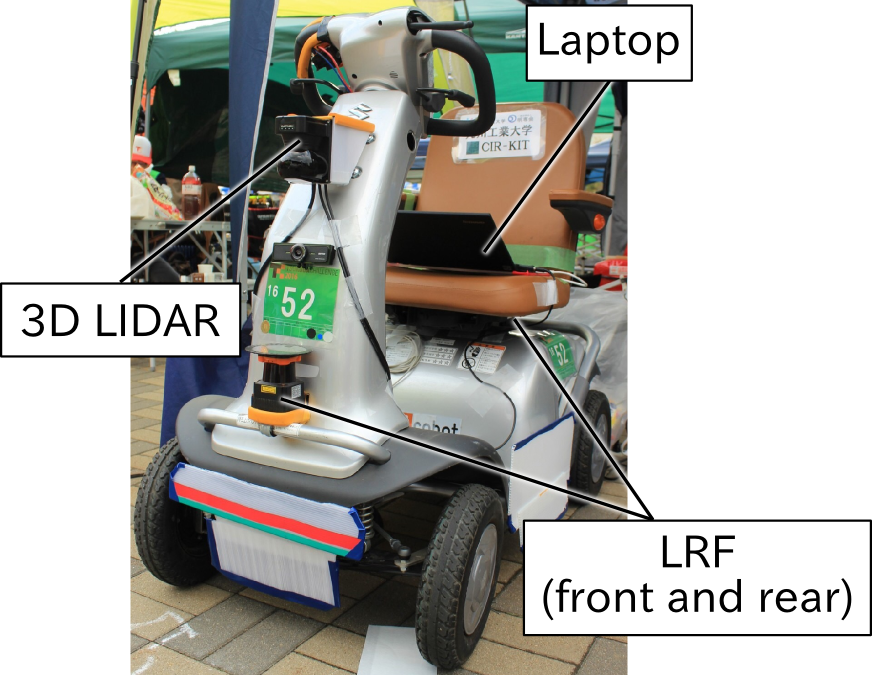
\includegraphics[width=6cm]{./fig/png/thirdrobot_2016ver.png}
 \caption{KIT-C3の全体図}
  \label{kitc3_robot}
\end{figure}


\subsubsection{センサ}
KIT-C3 は環境観測用センサとして前方下部に LRF (北陽電機製UTM-30LX)を1台,後方に同様のLRFを1台搭載している.探索対象の発見のために前方上部に3DLIDAR(北陽電機製YVT-X002)を1台取り付けた.また,ロボットの状態観測用センサとしてロータリーエンコーダ(MUTOH製UM-125)をステアリング軸に1つ取り付けている.このセニアカーの後輪は独立に2つのモータとエンコーダが搭載されており,そのエンコーダ情報をiXis Research社製マイコンボード iMCs01 により取得している.

\subsubsection{ロボットへの指令}
ロボットへの速度指令はロータリーエンコーダの処理用マイコンとして搭載した iXs Research 社のiMCs01を利用した.iMCs01で0-5[V]の電圧を生成しシニアカーのアクセル信号部に印加することで速度指令を実現している.またステアリング操舵のためのステッピングモータはArduino Unoを介して制御している.iMCs01とArduino Unoは制御用PCにUSBで接続し,制御用PCのOSはUbuntu 14.04を使用した.

\subsection{ソフトウェア構成}
\subsubsection{ROS}
ロボットの開発にはROS\cite{ros}を導入している.これはソフトウェアの再利用性を意識したものである.実際,KIT-C3で開発したソフトウェアを同チームが開発したKIT-C4やKIT-C5などの他のロボットでソフトウエア再利用することが可能であり,開発時間の短縮を図ることができる.また,ROSを用いることでデバッグや可視化に有効なツールだけでなく,世界中の開発者が作成したライブラリを容易に利用することができる.

\subsubsection{走行手法}
自律走行には,ROSのnavigationスタックを利用した.予め環境地図を作成し,環境地図上にWaypointを1メートル毎に設定し,それらを順に辿っていくようにして自律移動を行った.Waypointの設定はROSの可視化ソフトウェアrviz上でクリックやドラッグ操作で設定できるパッケージを開発しこれを用いた.経路生成および障害物回避にはmove\_baseパッケージを用いた.また,自己位置推定にはAMCL(AdaptiveMontecalro Localization)を用いた.今年も昨年と同様に前方と後方に取り付けた2台のLRFで自己位置推定を行った.また,グローバルパスプランニングにはcarrot\_planerを用いた.これはデフォルトのNavfnのグローバルプランナーでは人物発見の際に問題が生じたためである.また,ローカルプランナーにはDWAローカルプランナーを利用した.いずれも,ROSではmove\_baseのプラグインとして提供されているため簡単に利用することが出来る.
本番では人物探索を行うことが出来なかったが,人物探索についても準備を行った.予め設定したwaypointに探索エリアに関する情報を保持しておき,waypointの切替時に探索エリアかつ探索対象を発見して場合に探索対象候補へのアプローチを行った.探索対象の検出方法については\ref{200657_7Dec16}章で説明する.

\subsubsection{環境地図}
環境地図はROSのパッケージ化されたgmappingを用いて作成した.昨年は前後2台のLRFのデータを利用して地図作成を行ったが,今年は前方に取り付けたLRFのみで地図作成を行った.これはロボット後方のLRFの位置がつくば到着後に傾いたままデータを取ってしまったためである.環境地図は5[cm]四方の占有格子地図とした.また,確認走行を完了したあとは大清水公園と同公園の外でそれぞれ地図を作成し画像編集ソフトを用いて1つに統合したものを用いた.作成した地図は\ref{sec:remote_monitor}章のFig.\ref{monitor}に示す.遠隔監視システムの説明のために緑のマークが重ねてある.

\subsection{全体の構成}
これまでに説明した構成をFig.\ref{184559_7Dec16}にまとめた.ここで,ソフトウエアの枠の中には利用したROSのパッケージ群を掲載している.座標変換を行うtfなどは省略している.
\begin{figure*}[ht]
 \centering
 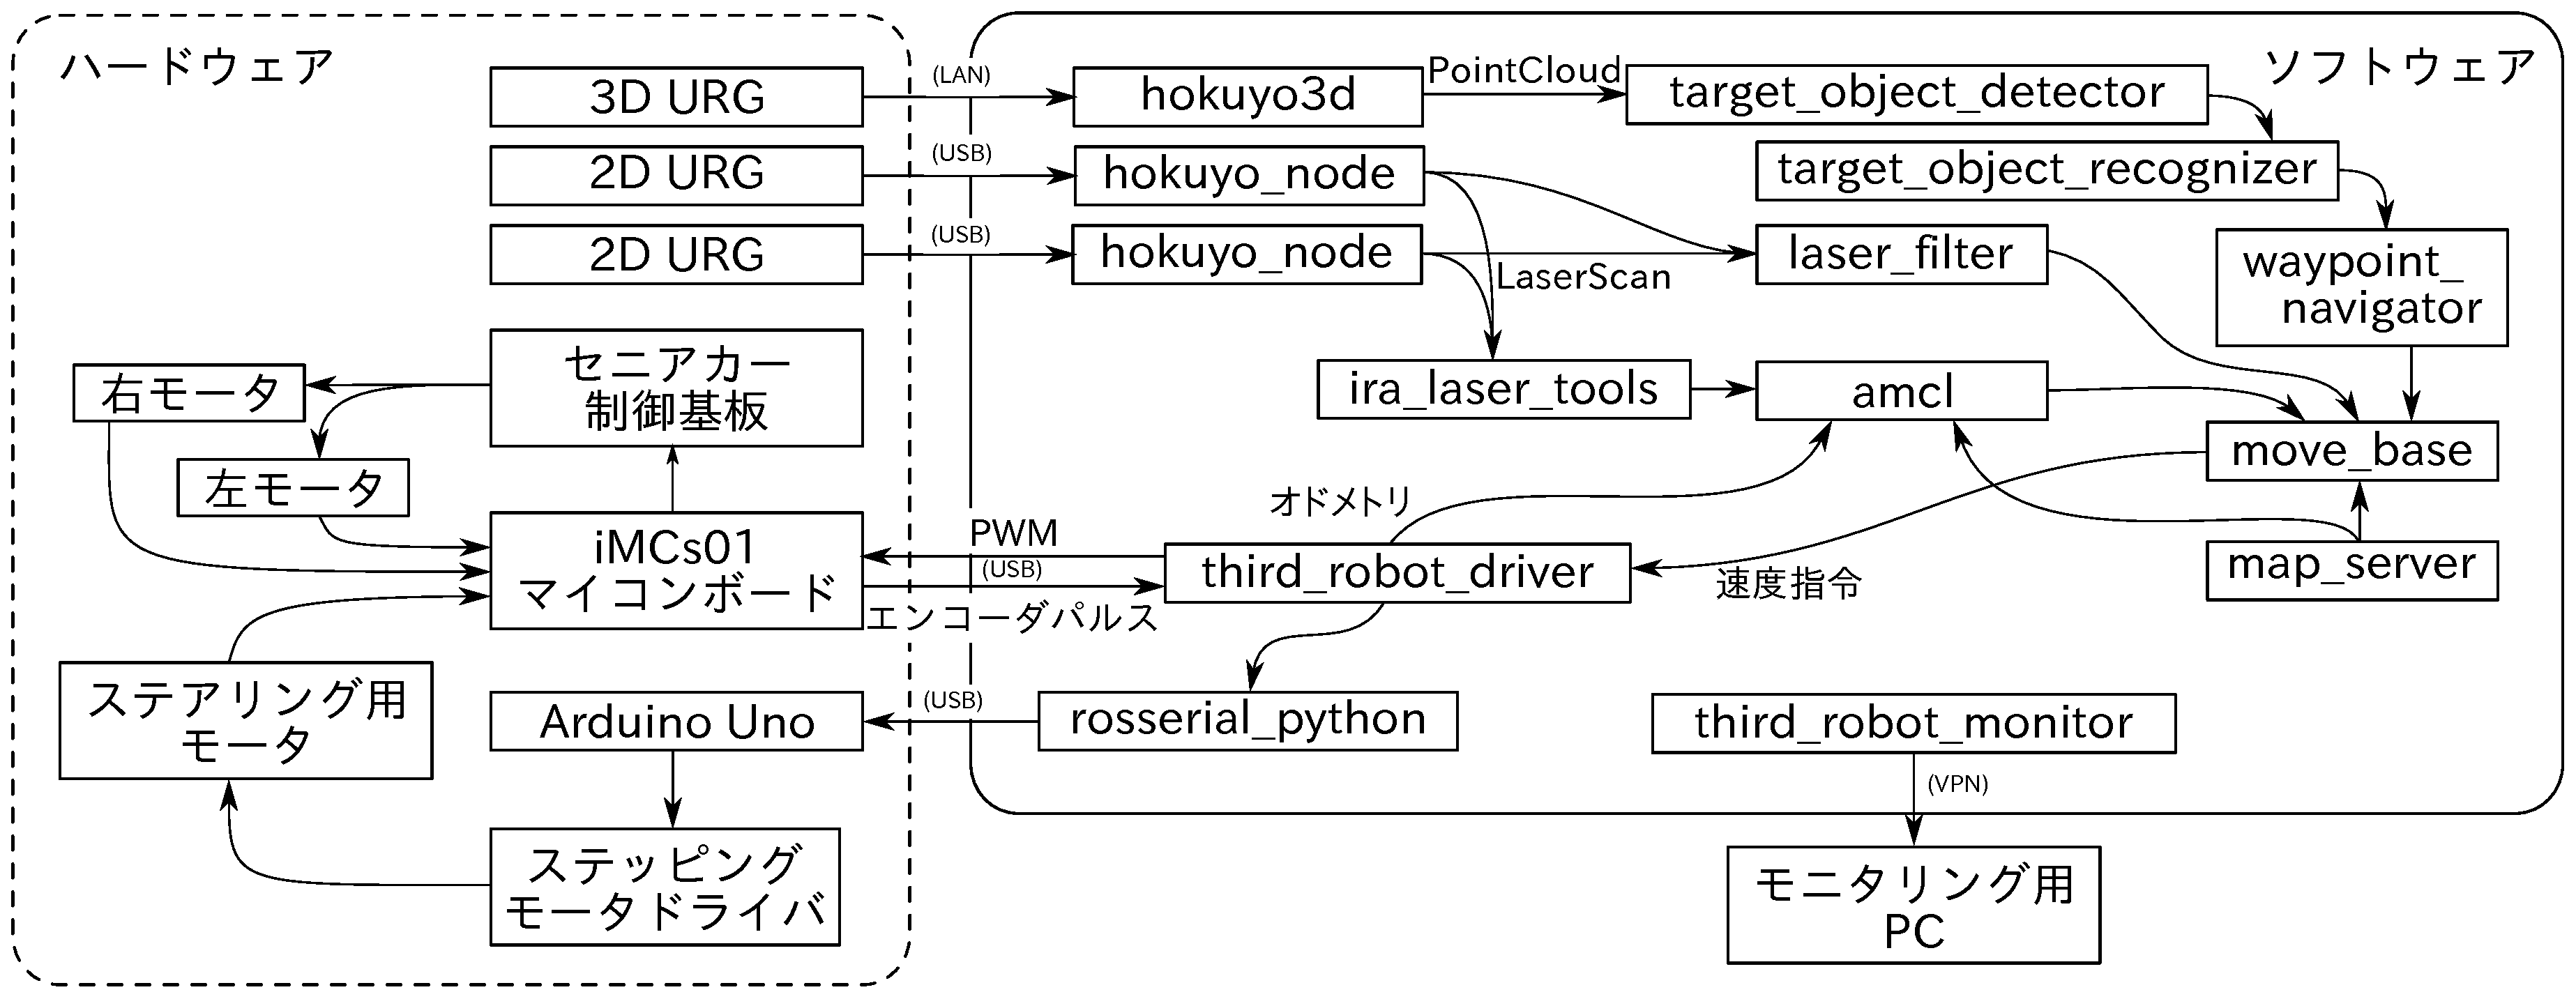
\includegraphics[width=16cm]{./fig/eps/whole_system.eps}
 \caption{KIT-C3の全体のシステム構成}
 \label{184559_7Dec16}
\end{figure*}

\end{document}

% Local Variables:
% mode: yatex
% TeX-master: "tc2016_third"
% End:
% 探索対象の発見課題に対する取り組み
\documentclass[10pt,a4paper]{jarticle}
\usepackage{docmute}
\usepackage{tc2016_utf}
\usepackage[dvipdfmx]{graphicx,color}
\usepackage[fleqn]{amsmath}
\usepackage{algorithm,algorithmic}
\usepackage{amssymb,epsfig}
\usepackage{ascmac}

\usepackage{url}
\usepackage{bm}
\usepackage{ascmac}
\usepackage{pifont}
%\usepackage{multirow}
\usepackage{enumerate}
%\usepackage{cases}
\usepackage{type1cm}
\usepackage{here}
\usepackage{secdot}
\sectiondot{subsection}
\sectiondot{subsubsection}

\DeclareRelationFont{JY1}{mc}{it}{}{OT1}{cmr}{it}{}
\DeclareRelationFont{JT1}{mc}{it}{}{OT1}{cmr}{it}{}
\DeclareFontShape{JY1}{mc}{m}{it}{<5> <6> <7> <8> <9> <10> sgen*min
    <10.95><12><14.4><17.28><20.74><24.88> min10
    <-> min10}{}
\DeclareFontShape{JT1}{mc}{m}{it}{<5> <6> <7> <8> <9> <10> sgen*tmin
    <10.95><12><14.4><17.28><20.74><24.88> tmin10
    <-> tmin10}{}
\DeclareRelationFont{JY1}{mc}{sl}{}{OT1}{cmr}{sl}{}
\DeclareRelationFont{JT1}{mc}{sl}{}{OT1}{cmr}{sl}{}
\DeclareFontShape{JY1}{mc}{m}{sl}{<5> <6> <7> <8> <9> <10> sgen*min
    <10.95><12><14.4><17.28><20.74><24.88> min10
    <-> min10}{}
\DeclareFontShape{JT1}{mc}{m}{sl}{<5> <6> <7> <8> <9> <10> sgen*tmin
    <10.95><12><14.4><17.28><20.74><24.88> tmin10
    <-> tmin10}{}
\DeclareRelationFont{JY1}{mc}{sc}{}{OT1}{cmr}{sc}{}
\DeclareRelationFont{JT1}{mc}{sc}{}{OT1}{cmr}{sc}{}
\DeclareFontShape{JY1}{mc}{m}{sc}{<5> <6> <7> <8> <9> <10> sgen*min
    <10.95><12><14.4><17.28><20.74><24.88> min10
    <-> min10}{}
\DeclareFontShape{JT1}{mc}{m}{sc}{<5> <6> <7> <8> <9> <10> sgen*tmin
    <10.95><12><14.4><17.28><20.74><24.88> tmin10
    <-> tmin10}{}
\DeclareRelationFont{JY1}{gt}{it}{}{OT1}{cmbx}{it}{}
\DeclareRelationFont{JT1}{gt}{it}{}{OT1}{cmbx}{it}{}
\DeclareFontShape{JY1}{mc}{bx}{it}{<5> <6> <7> <8> <9> <10> sgen*goth
    <10.95><12><14.4><17.28><20.74><24.88> goth10
    <-> goth10}{}
\DeclareFontShape{JT1}{mc}{bx}{it}{<5> <6> <7> <8> <9> <10> sgen*tgoth
    <10.95><12><14.4><17.28><20.74><24.88> tgoth10
    <-> tgoth10}{}
\DeclareRelationFont{JY1}{gt}{sl}{}{OT1}{cmbx}{sl}{}
\DeclareRelationFont{JT1}{gt}{sl}{}{OT1}{cmbx}{sl}{}
\DeclareFontShape{JY1}{mc}{bx}{sl}{<5> <6> <7> <8> <9> <10> sgen*goth
    <10.95><12><14.4><17.28><20.74><24.88> goth10
    <-> goth10}{}
\DeclareFontShape{JT1}{mc}{bx}{sl}{<5> <6> <7> <8> <9> <10> sgen*tgoth
    <10.95><12><14.4><17.28><20.74><24.88> tgoth10
    <-> tgoth10}{}
\DeclareRelationFont{JY1}{gt}{sc}{}{OT1}{cmbx}{sc}{}
\DeclareRelationFont{JT1}{gt}{sc}{}{OT1}{cmbx}{sc}{}
\DeclareFontShape{JY1}{mc}{bx}{sc}{<5> <6> <7> <8> <9> <10> sgen*goth
    <10.95><12><14.4><17.28><20.74><24.88> goth10
    <-> goth10}{}
\DeclareFontShape{JT1}{mc}{bx}{sc}{<5> <6> <7> <8> <9> <10> sgen*tgoth
    <10.95><12><14.4><17.28><20.74><24.88> tgoth10
    <-> tgoth10}{}
\DeclareRelationFont{JY1}{gt}{it}{}{OT1}{cmr}{it}{}
\DeclareRelationFont{JT1}{gt}{it}{}{OT1}{cmr}{it}{}
\DeclareFontShape{JY1}{gt}{m}{it}{<5> <6> <7> <8> <9> <10> sgen*goth
    <10.95><12><14.4><17.28><20.74><24.88> goth10
    <-> goth10}{}
\DeclareFontShape{JT1}{gt}{m}{it}{<5> <6> <7> <8> <9> <10> sgen*tgoth
    <10.95><12><14.4><17.28><20.74><24.88> tgoth10
    <-> tgoth10}{}
\endinput
%%%% end of jdummy.def

\def\vec#1{\mbox{\boldmath$#1$}}
\def\vector#1{\mbox{\boldmath $#1$}}

\newcommand{\argmax}{\mathop{\rm arg~max}\limits}
\newcommand{\argmin}{\mathop{\rm arg~min}\limits}
\newcommand{\umax}{\mathop{\rm max}\limits}

\def\R{{\Bbb R}}
\def\Z{{\Bbb Z}}

\renewcommand{\topfraction}{0.8}
\renewcommand{\bottomfraction}{0.8}
\renewcommand{\dbltopfraction}{0.8}
\renewcommand{\textfraction}{0.1}
\renewcommand{\floatpagefraction}{0.8}
\renewcommand{\dblfloatpagefraction}{0.8}
\setcounter{topnumber}{3}
\setcounter{bottomnumber}{3}
\setcounter{totalnumber}{3}
\begin{document}
\section{探索対象の発見課題に対する取り組み}
\label{200657_7Dec16}
課題コース途中で探索エリアにおいて特定人物(探索対象)の発見という課題も設定されている.我々はこの課題を3次元LIDARから得られた3次元点群の処理による実現を試みた.

\subsection{地面点群の除去}
3次元LIDAR(Hokuyo YVT-X002)で得られた3次元点群からまず地面点群の除去を行う.LIDARの取り付け位置は既知であり,つくばチャレンジ2016の課題コースでは探索エリアは平面だったため,地面点群はZ方向の高さによって消去した.
\subsection{クラスタリング}
地面点群が除去された点群をユークリディアンクラスタリングによりクラスタリングを行った.ユークリディアンクラスタリングではある点群からのユークリッド距離がしきい値以下の場合に同一クラスタとする手法である.
\subsection{識別}
クラスタリング後の点群の識別には夏迫ら\cite{chibainst2015}がつくばチャレンジ2015のレポートで提案されていた手法を参考にSVMによる手法を利用した.しかし,特徴量に関しては文献\cite{城殿清澄2011高解像度レーザレーダによる歩行者識別}\cite{liukun2015}\cite{tokudome2016}の特徴量を用いた.
\subsubsection{点群特徴量}
識別に利用した特徴量$f_{i}$は6次元からなる$f_{i1}$と7次元からなる$f_{i2}$の2つの特徴ベクトルを並べた13次元の特徴量である.
まず,$f_{i1}$は点群の3次元共分散行列の要素であり次式で示される.
\begin{eqnarray}
 \Sigma = \frac{1}{n-1}\sum_{\vec{x_{k}}(i)\in C_{i}}\vec{x}_{k}^{(i)}\vec{x}_{k}^{(i)T}\label{234310_5Dec16}
\end{eqnarray}
ここで,$\vec{x}_{k}^{(i)}\triangleq[x_{k}^{(i)} y_{k}^{(i)} z_{k}^{(i)}]^{T}$はクラスタ内に含まれる点群のクラスタ重心を原点とする座標である.この行列は対称行列であるため,行列要素のうち重複を除いた6要素を特徴量として,$\vec{f}_{i1} = [f_{i11}, \cdots, f_{i16}]^{T}$とする.
式\eqref{234310_5Dec16}に示す3次元共分散行列の固有値を$\lambda_{1}, \lambda_{2}, \lambda_{3}$とする.ただし,$\lambda_{1} < \lambda_{2} < \lambda_{3}$である.この固有値を元にTable.\ref{222525_5Dec16}に示す特徴量を計算しこれを$\vec{f}_{i2}$とした.
\begin{table}
 \centering
 \caption{3D features of points}
 \label{222525_5Dec16}
 \begin{tabular}{|c|c|c|}
  \hline
  $f_{i21}$ & Linearity & $(\lambda_{1}-\lambda_{2})/\lambda_{1}$ \\
  $f_{i22}$ & Planarity & $(\lambda_{2}-\lambda_{3})/\lambda_{1}$ \\
  $f_{i23}$ & Scattering & $\lambda_{3}/\lambda_{1}$ \\
  $f_{i24}$ & Omnivariance & $\sqrt[3]{\lambda_{1}\lambda_{2}\lambda_{3}}$ \\
  $f_{i25}$ & Anisotropy & $(\lambda_{1}-\lambda_{3})/\lambda_{1}$ \\
  $f_{i26}$ & Eigenetropy & $-\sum^{3}_{i=1}\lambda_{i}\ln\lambda_{i}$ \\
  $f_{i27}$ & Change of curvature & $\lambda_{3}/(\lambda_{1}+\lambda_{2}+\lambda_{3})$ \\
  \hline
 \end{tabular}
\end{table}

\subsubsection{SVM}
得られた特徴量をSVM(Support Vector Machine)を用いて識別する.実装にはLIBSVMを利用した.学習はクラスタリングによって得られた点群を287個用意して,それらを探索対象とその他の2値分類問題として行った.学習の結果訓練データで99.3\%,テストデータでも85\%の精度が得られた.

\subsection{探索対象へのアプローチ}
実用上は学習データ数が少なかったこともあり,誤検出が多くなってしまった.そこで,検出位置から1メートル以内で複数回,探索対象と認識した場合にのみアプローチすることにした.
探索対象が見つかった場合には,Fig.\ref{142629_6Dec16}のように探索対象を中心とする円とロボットの自己位置と探索対象を直線結んだ時の交点座標のうち,ロボットに近い方の交点を新たなゴールとして設定する.

\begin{figure}[ht]
 \centering
 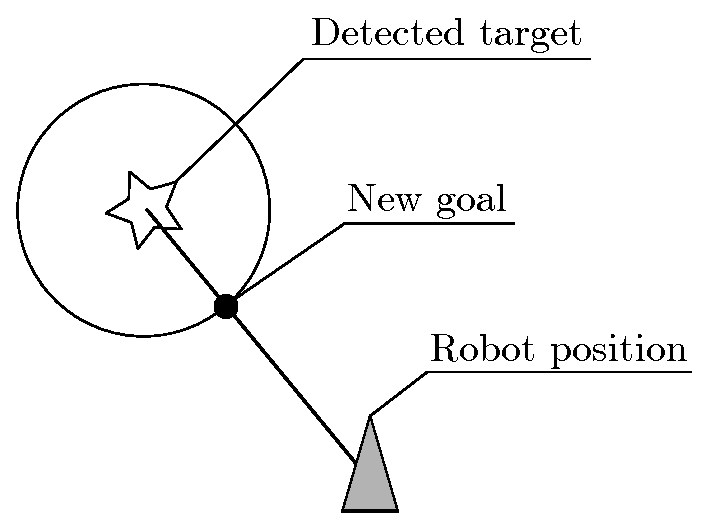
\includegraphics[width=5cm]{./fig/eps/approach_to_target.eps}
 \caption{探索対象へのアプローチ}
 \label{142629_6Dec16}
\end{figure}

以下にこれまでに述べた手法をまとめる.
\begin{enumerate}
 \item 3DLIDARによって得られた点群から地面点群を除去する
 \item 地面点群が除去された点群をクラスタリングする
 \item クラスタリング結果をSVMによって識別し,探索対象ならアプローチ候補とする
 \item アプローチ候補のうち,1m以内で複数回アプローチ候補が検出された場合にアプローチ対象とする
\end{enumerate}

\subsubsection{人物探索のつくばチャレンジにおける実験結果}
これまでに説明した手法は九州工業大学戸畑キャンパス内に設定したコース内では実用に耐える精度で機能していた.しかし,試験走行日にこれらを実際に試してみたところ,学内で実験した場合よりも多く誤認識してしまい,それら全てにアプローチを試みるという結果になってしまった.そのため,制限時間内で課題コースを完走することが難しいと判断し,本走行では人物探索機能を起動させなかった.
課題コースでは建物の角などを探索対象として多く誤認識してしまっていた.学内で得られたサンプルには建物の角など人工物があまり含まれておらず,結果としてそれらを上手く識別できていなかったと考えられる.すなわち,学習に用いたデータが少なすぎたことが問題だと考えられる.

\end{document}

% Local Variables:
% mode: yatex
% TeX-master: "tc2016_third.tex"
% End:

% 遠隔監視システム
\documentclass[10pt,a4paper]{jarticle}
\usepackage{docmute}
\usepackage{tc2016_utf}
\usepackage[dvipdfmx]{graphicx,color}
\usepackage[fleqn]{amsmath}
\usepackage{algorithm,algorithmic}
\usepackage{amssymb,epsfig}
\usepackage{ascmac}

\usepackage{url}
\usepackage{bm}
\usepackage{ascmac}
\usepackage{pifont}
%\usepackage{multirow}
\usepackage{enumerate}
%\usepackage{cases}
\usepackage{type1cm}
\usepackage{here}
\usepackage{secdot}
\sectiondot{subsection}
\sectiondot{subsubsection}

\DeclareRelationFont{JY1}{mc}{it}{}{OT1}{cmr}{it}{}
\DeclareRelationFont{JT1}{mc}{it}{}{OT1}{cmr}{it}{}
\DeclareFontShape{JY1}{mc}{m}{it}{<5> <6> <7> <8> <9> <10> sgen*min
    <10.95><12><14.4><17.28><20.74><24.88> min10
    <-> min10}{}
\DeclareFontShape{JT1}{mc}{m}{it}{<5> <6> <7> <8> <9> <10> sgen*tmin
    <10.95><12><14.4><17.28><20.74><24.88> tmin10
    <-> tmin10}{}
\DeclareRelationFont{JY1}{mc}{sl}{}{OT1}{cmr}{sl}{}
\DeclareRelationFont{JT1}{mc}{sl}{}{OT1}{cmr}{sl}{}
\DeclareFontShape{JY1}{mc}{m}{sl}{<5> <6> <7> <8> <9> <10> sgen*min
    <10.95><12><14.4><17.28><20.74><24.88> min10
    <-> min10}{}
\DeclareFontShape{JT1}{mc}{m}{sl}{<5> <6> <7> <8> <9> <10> sgen*tmin
    <10.95><12><14.4><17.28><20.74><24.88> tmin10
    <-> tmin10}{}
\DeclareRelationFont{JY1}{mc}{sc}{}{OT1}{cmr}{sc}{}
\DeclareRelationFont{JT1}{mc}{sc}{}{OT1}{cmr}{sc}{}
\DeclareFontShape{JY1}{mc}{m}{sc}{<5> <6> <7> <8> <9> <10> sgen*min
    <10.95><12><14.4><17.28><20.74><24.88> min10
    <-> min10}{}
\DeclareFontShape{JT1}{mc}{m}{sc}{<5> <6> <7> <8> <9> <10> sgen*tmin
    <10.95><12><14.4><17.28><20.74><24.88> tmin10
    <-> tmin10}{}
\DeclareRelationFont{JY1}{gt}{it}{}{OT1}{cmbx}{it}{}
\DeclareRelationFont{JT1}{gt}{it}{}{OT1}{cmbx}{it}{}
\DeclareFontShape{JY1}{mc}{bx}{it}{<5> <6> <7> <8> <9> <10> sgen*goth
    <10.95><12><14.4><17.28><20.74><24.88> goth10
    <-> goth10}{}
\DeclareFontShape{JT1}{mc}{bx}{it}{<5> <6> <7> <8> <9> <10> sgen*tgoth
    <10.95><12><14.4><17.28><20.74><24.88> tgoth10
    <-> tgoth10}{}
\DeclareRelationFont{JY1}{gt}{sl}{}{OT1}{cmbx}{sl}{}
\DeclareRelationFont{JT1}{gt}{sl}{}{OT1}{cmbx}{sl}{}
\DeclareFontShape{JY1}{mc}{bx}{sl}{<5> <6> <7> <8> <9> <10> sgen*goth
    <10.95><12><14.4><17.28><20.74><24.88> goth10
    <-> goth10}{}
\DeclareFontShape{JT1}{mc}{bx}{sl}{<5> <6> <7> <8> <9> <10> sgen*tgoth
    <10.95><12><14.4><17.28><20.74><24.88> tgoth10
    <-> tgoth10}{}
\DeclareRelationFont{JY1}{gt}{sc}{}{OT1}{cmbx}{sc}{}
\DeclareRelationFont{JT1}{gt}{sc}{}{OT1}{cmbx}{sc}{}
\DeclareFontShape{JY1}{mc}{bx}{sc}{<5> <6> <7> <8> <9> <10> sgen*goth
    <10.95><12><14.4><17.28><20.74><24.88> goth10
    <-> goth10}{}
\DeclareFontShape{JT1}{mc}{bx}{sc}{<5> <6> <7> <8> <9> <10> sgen*tgoth
    <10.95><12><14.4><17.28><20.74><24.88> tgoth10
    <-> tgoth10}{}
\DeclareRelationFont{JY1}{gt}{it}{}{OT1}{cmr}{it}{}
\DeclareRelationFont{JT1}{gt}{it}{}{OT1}{cmr}{it}{}
\DeclareFontShape{JY1}{gt}{m}{it}{<5> <6> <7> <8> <9> <10> sgen*goth
    <10.95><12><14.4><17.28><20.74><24.88> goth10
    <-> goth10}{}
\DeclareFontShape{JT1}{gt}{m}{it}{<5> <6> <7> <8> <9> <10> sgen*tgoth
    <10.95><12><14.4><17.28><20.74><24.88> tgoth10
    <-> tgoth10}{}
\endinput
%%%% end of jdummy.def

\def\vec#1{\mbox{\boldmath$#1$}}
\def\vector#1{\mbox{\boldmath $#1$}}

\newcommand{\argmax}{\mathop{\rm arg~max}\limits}
\newcommand{\argmin}{\mathop{\rm arg~min}\limits}
\newcommand{\umax}{\mathop{\rm max}\limits}

\def\R{{\Bbb R}}
\def\Z{{\Bbb Z}}

\renewcommand{\topfraction}{0.8}
\renewcommand{\bottomfraction}{0.8}
\renewcommand{\dbltopfraction}{0.8}
\renewcommand{\textfraction}{0.1}
\renewcommand{\floatpagefraction}{0.8}
\renewcommand{\dblfloatpagefraction}{0.8}
\setcounter{topnumber}{3}
\setcounter{bottomnumber}{3}
\setcounter{totalnumber}{3}
\begin{document}
\section{遠隔監視システム}
\label{sec:remote_monitor}
つくばチャレンジの注意事項等について,「ロボットの位置や状況のステーションにおけるモニタリング」を強く推奨すると明記されている.我々は本要求事項を達成する遠隔監視システムを構築し,九州からつくばでのロボットの遠隔監視に成功した.その機能とネットワーク環境について述べる.

まず監視画面として,ロボットの現在姿勢を地図上にリアルタイムに表示させる形式を採用した.実験走行時に現在姿勢の全履歴を表示した様子をFig.\ref{monitor}に示す.スタートからゴールまでの経路が表示されていることが確認できる.加えて,探索対象アプローチ位置も同時に表示できるようにした.

\begin{figure}
    \centering
    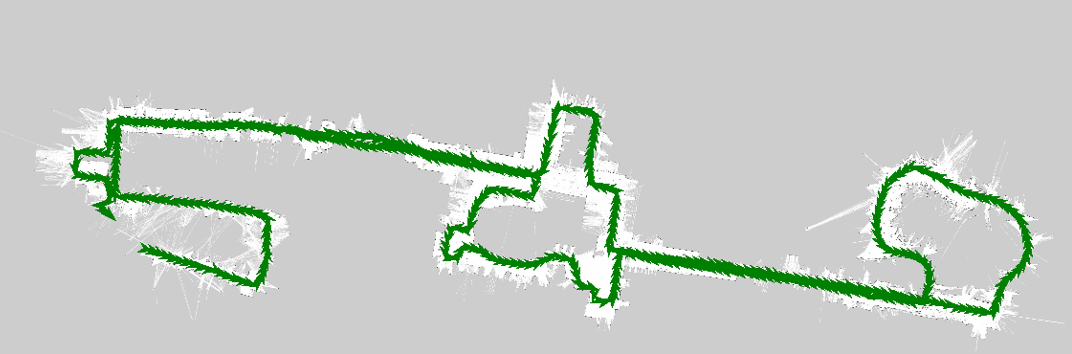
\includegraphics[width=8cm]{fig/png/monitor.png}
    \caption{遠隔監視システムで地図上に現在姿勢を表示させた様子.}
    \label{monitor}
\end{figure}

次に,通信環境について述べる.監視端末とロボット間の通信回線として商用モバイル回線を利用し,OpenVPN \cite{openvpn} による遠隔通信を採用した.遠隔監視PCをサーバ,ロボットをクライアントとしてVPNネットワークを構成し,ROS ネットワークと連携させることで,遠隔監視を実現した.

工夫点としては,ロボットが一定距離を移動する毎に,自身の位置を監視端末に送信する仕様とした点が挙げられる.モバイル回線でOpenVPNを利用するという制約があるため,通信容量を節減することが目的である.実験走行では送信間隔を5[m]に設定したところ,通信容量を大幅に低減することに成功した.

\end{document}

% Local Variables:
% mode: yatex
% TeX-master: "tc2016_third"
% End:

% つくばチャレンジ2016の結果と考察
\documentclass[10pt,a4paper]{jarticle}
\usepackage{docmute}
\usepackage{tc2016_utf}
\usepackage[dvipdfmx]{graphicx,color}
\usepackage[fleqn]{amsmath}
\usepackage{algorithm,algorithmic}
\usepackage{amssymb,epsfig}
\usepackage{ascmac}

\usepackage{url}
\usepackage{bm}
\usepackage{ascmac}
\usepackage{pifont}
%\usepackage{multirow}
\usepackage{enumerate}
%\usepackage{cases}
\usepackage{type1cm}
\usepackage{here}
\usepackage{secdot}
\sectiondot{subsection}
\sectiondot{subsubsection}

\DeclareRelationFont{JY1}{mc}{it}{}{OT1}{cmr}{it}{}
\DeclareRelationFont{JT1}{mc}{it}{}{OT1}{cmr}{it}{}
\DeclareFontShape{JY1}{mc}{m}{it}{<5> <6> <7> <8> <9> <10> sgen*min
    <10.95><12><14.4><17.28><20.74><24.88> min10
    <-> min10}{}
\DeclareFontShape{JT1}{mc}{m}{it}{<5> <6> <7> <8> <9> <10> sgen*tmin
    <10.95><12><14.4><17.28><20.74><24.88> tmin10
    <-> tmin10}{}
\DeclareRelationFont{JY1}{mc}{sl}{}{OT1}{cmr}{sl}{}
\DeclareRelationFont{JT1}{mc}{sl}{}{OT1}{cmr}{sl}{}
\DeclareFontShape{JY1}{mc}{m}{sl}{<5> <6> <7> <8> <9> <10> sgen*min
    <10.95><12><14.4><17.28><20.74><24.88> min10
    <-> min10}{}
\DeclareFontShape{JT1}{mc}{m}{sl}{<5> <6> <7> <8> <9> <10> sgen*tmin
    <10.95><12><14.4><17.28><20.74><24.88> tmin10
    <-> tmin10}{}
\DeclareRelationFont{JY1}{mc}{sc}{}{OT1}{cmr}{sc}{}
\DeclareRelationFont{JT1}{mc}{sc}{}{OT1}{cmr}{sc}{}
\DeclareFontShape{JY1}{mc}{m}{sc}{<5> <6> <7> <8> <9> <10> sgen*min
    <10.95><12><14.4><17.28><20.74><24.88> min10
    <-> min10}{}
\DeclareFontShape{JT1}{mc}{m}{sc}{<5> <6> <7> <8> <9> <10> sgen*tmin
    <10.95><12><14.4><17.28><20.74><24.88> tmin10
    <-> tmin10}{}
\DeclareRelationFont{JY1}{gt}{it}{}{OT1}{cmbx}{it}{}
\DeclareRelationFont{JT1}{gt}{it}{}{OT1}{cmbx}{it}{}
\DeclareFontShape{JY1}{mc}{bx}{it}{<5> <6> <7> <8> <9> <10> sgen*goth
    <10.95><12><14.4><17.28><20.74><24.88> goth10
    <-> goth10}{}
\DeclareFontShape{JT1}{mc}{bx}{it}{<5> <6> <7> <8> <9> <10> sgen*tgoth
    <10.95><12><14.4><17.28><20.74><24.88> tgoth10
    <-> tgoth10}{}
\DeclareRelationFont{JY1}{gt}{sl}{}{OT1}{cmbx}{sl}{}
\DeclareRelationFont{JT1}{gt}{sl}{}{OT1}{cmbx}{sl}{}
\DeclareFontShape{JY1}{mc}{bx}{sl}{<5> <6> <7> <8> <9> <10> sgen*goth
    <10.95><12><14.4><17.28><20.74><24.88> goth10
    <-> goth10}{}
\DeclareFontShape{JT1}{mc}{bx}{sl}{<5> <6> <7> <8> <9> <10> sgen*tgoth
    <10.95><12><14.4><17.28><20.74><24.88> tgoth10
    <-> tgoth10}{}
\DeclareRelationFont{JY1}{gt}{sc}{}{OT1}{cmbx}{sc}{}
\DeclareRelationFont{JT1}{gt}{sc}{}{OT1}{cmbx}{sc}{}
\DeclareFontShape{JY1}{mc}{bx}{sc}{<5> <6> <7> <8> <9> <10> sgen*goth
    <10.95><12><14.4><17.28><20.74><24.88> goth10
    <-> goth10}{}
\DeclareFontShape{JT1}{mc}{bx}{sc}{<5> <6> <7> <8> <9> <10> sgen*tgoth
    <10.95><12><14.4><17.28><20.74><24.88> tgoth10
    <-> tgoth10}{}
\DeclareRelationFont{JY1}{gt}{it}{}{OT1}{cmr}{it}{}
\DeclareRelationFont{JT1}{gt}{it}{}{OT1}{cmr}{it}{}
\DeclareFontShape{JY1}{gt}{m}{it}{<5> <6> <7> <8> <9> <10> sgen*goth
    <10.95><12><14.4><17.28><20.74><24.88> goth10
    <-> goth10}{}
\DeclareFontShape{JT1}{gt}{m}{it}{<5> <6> <7> <8> <9> <10> sgen*tgoth
    <10.95><12><14.4><17.28><20.74><24.88> tgoth10
    <-> tgoth10}{}
\endinput
%%%% end of jdummy.def

\def\vec#1{\mbox{\boldmath$#1$}}
\def\vector#1{\mbox{\boldmath $#1$}}

\newcommand{\argmax}{\mathop{\rm arg~max}\limits}
\newcommand{\argmin}{\mathop{\rm arg~min}\limits}
\newcommand{\umax}{\mathop{\rm max}\limits}

\def\R{{\Bbb R}}
\def\Z{{\Bbb Z}}

\renewcommand{\topfraction}{0.8}
\renewcommand{\bottomfraction}{0.8}
\renewcommand{\dbltopfraction}{0.8}
\renewcommand{\textfraction}{0.1}
\renewcommand{\floatpagefraction}{0.8}
\renewcommand{\dblfloatpagefraction}{0.8}
\setcounter{topnumber}{3}
\setcounter{bottomnumber}{3}
\setcounter{totalnumber}{3}
\begin{document}
\section{つくばチャレンジ2016の結果と考察}
\subsection{実験走行}
横断歩道には挑戦しなかった。これは我々のチームがこれまで完走を達成出来たことが無かったため,まずは完走を目指したためである.
中央公園後半付近ではランドマークになるものが少なく,上手く地図作成出来ず,実験走行では自律走行に失敗することがあった.

\subsection{本走行結果}
本走行の結果,横断歩道を除く課題コースの全区間を完走することが出来た.また,人物探索を行うような走行経路を通ったが人物探索は行っていない.実験走行で上手く機能しないことが判明したためである.
不安定だった中央公園の後半付近の地図を本走行の前に取り直すことで,奔走では完走を達成できた.一方で,オドメトリの向上を行い,ランドマークが無い環境でも安定して地図作成が出来るような仕組みを取り入れる必要があると考えられる.


\end{document}
% その他(開発状況,筑波での流れ,謝辞など)
\documentclass[10pt,a4paper]{jarticle}
\usepackage{docmute}
\usepackage{tc2016_utf}
\usepackage[dvipdfmx]{graphicx,color}
\usepackage[fleqn]{amsmath}
\usepackage{algorithm,algorithmic}
\usepackage{amssymb,epsfig}
\usepackage{ascmac}

\usepackage{url}
\usepackage{bm}
\usepackage{ascmac}
\usepackage{pifont}
%\usepackage{multirow}
\usepackage{enumerate}
%\usepackage{cases}
\usepackage{type1cm}
\usepackage{here}
\usepackage{secdot}
\sectiondot{subsection}
\sectiondot{subsubsection}

\DeclareRelationFont{JY1}{mc}{it}{}{OT1}{cmr}{it}{}
\DeclareRelationFont{JT1}{mc}{it}{}{OT1}{cmr}{it}{}
\DeclareFontShape{JY1}{mc}{m}{it}{<5> <6> <7> <8> <9> <10> sgen*min
    <10.95><12><14.4><17.28><20.74><24.88> min10
    <-> min10}{}
\DeclareFontShape{JT1}{mc}{m}{it}{<5> <6> <7> <8> <9> <10> sgen*tmin
    <10.95><12><14.4><17.28><20.74><24.88> tmin10
    <-> tmin10}{}
\DeclareRelationFont{JY1}{mc}{sl}{}{OT1}{cmr}{sl}{}
\DeclareRelationFont{JT1}{mc}{sl}{}{OT1}{cmr}{sl}{}
\DeclareFontShape{JY1}{mc}{m}{sl}{<5> <6> <7> <8> <9> <10> sgen*min
    <10.95><12><14.4><17.28><20.74><24.88> min10
    <-> min10}{}
\DeclareFontShape{JT1}{mc}{m}{sl}{<5> <6> <7> <8> <9> <10> sgen*tmin
    <10.95><12><14.4><17.28><20.74><24.88> tmin10
    <-> tmin10}{}
\DeclareRelationFont{JY1}{mc}{sc}{}{OT1}{cmr}{sc}{}
\DeclareRelationFont{JT1}{mc}{sc}{}{OT1}{cmr}{sc}{}
\DeclareFontShape{JY1}{mc}{m}{sc}{<5> <6> <7> <8> <9> <10> sgen*min
    <10.95><12><14.4><17.28><20.74><24.88> min10
    <-> min10}{}
\DeclareFontShape{JT1}{mc}{m}{sc}{<5> <6> <7> <8> <9> <10> sgen*tmin
    <10.95><12><14.4><17.28><20.74><24.88> tmin10
    <-> tmin10}{}
\DeclareRelationFont{JY1}{gt}{it}{}{OT1}{cmbx}{it}{}
\DeclareRelationFont{JT1}{gt}{it}{}{OT1}{cmbx}{it}{}
\DeclareFontShape{JY1}{mc}{bx}{it}{<5> <6> <7> <8> <9> <10> sgen*goth
    <10.95><12><14.4><17.28><20.74><24.88> goth10
    <-> goth10}{}
\DeclareFontShape{JT1}{mc}{bx}{it}{<5> <6> <7> <8> <9> <10> sgen*tgoth
    <10.95><12><14.4><17.28><20.74><24.88> tgoth10
    <-> tgoth10}{}
\DeclareRelationFont{JY1}{gt}{sl}{}{OT1}{cmbx}{sl}{}
\DeclareRelationFont{JT1}{gt}{sl}{}{OT1}{cmbx}{sl}{}
\DeclareFontShape{JY1}{mc}{bx}{sl}{<5> <6> <7> <8> <9> <10> sgen*goth
    <10.95><12><14.4><17.28><20.74><24.88> goth10
    <-> goth10}{}
\DeclareFontShape{JT1}{mc}{bx}{sl}{<5> <6> <7> <8> <9> <10> sgen*tgoth
    <10.95><12><14.4><17.28><20.74><24.88> tgoth10
    <-> tgoth10}{}
\DeclareRelationFont{JY1}{gt}{sc}{}{OT1}{cmbx}{sc}{}
\DeclareRelationFont{JT1}{gt}{sc}{}{OT1}{cmbx}{sc}{}
\DeclareFontShape{JY1}{mc}{bx}{sc}{<5> <6> <7> <8> <9> <10> sgen*goth
    <10.95><12><14.4><17.28><20.74><24.88> goth10
    <-> goth10}{}
\DeclareFontShape{JT1}{mc}{bx}{sc}{<5> <6> <7> <8> <9> <10> sgen*tgoth
    <10.95><12><14.4><17.28><20.74><24.88> tgoth10
    <-> tgoth10}{}
\DeclareRelationFont{JY1}{gt}{it}{}{OT1}{cmr}{it}{}
\DeclareRelationFont{JT1}{gt}{it}{}{OT1}{cmr}{it}{}
\DeclareFontShape{JY1}{gt}{m}{it}{<5> <6> <7> <8> <9> <10> sgen*goth
    <10.95><12><14.4><17.28><20.74><24.88> goth10
    <-> goth10}{}
\DeclareFontShape{JT1}{gt}{m}{it}{<5> <6> <7> <8> <9> <10> sgen*tgoth
    <10.95><12><14.4><17.28><20.74><24.88> tgoth10
    <-> tgoth10}{}
\endinput
%%%% end of jdummy.def

\def\vec#1{\mbox{\boldmath$#1$}}
\def\vector#1{\mbox{\boldmath $#1$}}

\newcommand{\argmax}{\mathop{\rm arg~max}\limits}
\newcommand{\argmin}{\mathop{\rm arg~min}\limits}
\newcommand{\umax}{\mathop{\rm max}\limits}

\def\R{{\Bbb R}}
\def\Z{{\Bbb Z}}

\renewcommand{\topfraction}{0.8}
\renewcommand{\bottomfraction}{0.8}
\renewcommand{\dbltopfraction}{0.8}
\renewcommand{\textfraction}{0.1}
\renewcommand{\floatpagefraction}{0.8}
\renewcommand{\dblfloatpagefraction}{0.8}
\setcounter{topnumber}{3}
\setcounter{bottomnumber}{3}
\setcounter{totalnumber}{3}
\begin{document}

\section{開発状況などに関して}
本年度の開発では,昨年度までに開発してきたロボットを用いた.開発を行うにあたり,我々のチームは実験走行になかなか参加出来ないため,学内での実験を積み重ねてきた.学内の実験においても約1000[m]程度の自律走行が安定してできていた.しかし,学内での実験では他のロボットや歩行者などの未知の障害物などが少なく,それらを想定した実験を行う必要があった.

\section{つくばでの実験の流れ}
\begin{description}
 \item[11月○○日]\mbox{}\\
	    ロボットやテントなどを梱包
 \item[11月○○日]\mbox{}\\
	    ロボットや機材などを搬送業者に引き渡し
 \item[11月○○日]\mbox{}\\
	    つくば市着 ロボットの準備
 \item[11月○○日]\mbox{}\\
	    第○回実験走行 ロボットの安全確認、大清水公園のデータ取得、大清水公園の地図作成、ウェイポイントの設定,大清水公園の自律走行,確認走行,課題コース全体のデータ取得を行った
 \item[11月○○日]\mbox{}\\
	    第○回実験走行 課題コース全体のテスト走行、探索対象の発見及びアプローチの実験,遠隔監視システムの動作確認
 \item[11月○○日]\mbox{}\\
	    本走行 朝の走行実験で第○回実験走行で上手く自律走行出来なかった箇所の地図を再度取得。ウェイポイントの再設定。交流会終了後、ロボット等の梱包
 \item[11月○○日]\mbox{}\\
	    北九州着
\end{description}
つくばチャレンジに遠方から参加する場合,なかなか実験走行に参加できないため,実験走行日にどれだけ実験できるかどうかが重要になってくる。

\section{最後に}
我々が開発したソースコードは,GitHub上で公開している.開発を行うにあたって参考にしていただければありがたい.
\url{http://github.com/Nishida-Lab/TC2015}

\section*{謝辞}
つくばチャレンジ実行委員会やつくば市の方々にはつくばチャレンジのような貴重な実験の機会を与えていただき感謝いたします.
\end{document}

% Local Variables:
% mode: yatex
% TeX-master: "tc2016_third"
% End:

\bibliographystyle{IEEEtran}
\bibliography{tc2016_third}

%\appendix
%\section{}

\end{document}
